Our project is about \textit{Question Answering}, a field of research included in \textit{Natural Language Processing} (NLP) theory. NLP mixes linguistic and computer science and is made of all kinds of automated techniques that have to deal with natural languages, such as French or English. For instance, automatic translation or text summarization are also parts of NLP.

In Natural Language Processing, sentences are often represented in a condensed and normalized form called \textit{(subject, predicate, object) triple representation}. For example, the phrase ``Fleming discovered penicillin.'' will be represented by the triple (penicillin, discoverer, Fleming). Two triples can be associated to ``The president was born in 1950 and died in 2000.'': (president, birth date, 1950) and (president, death date, 2000). This representation has been formalized into the \textit{Resource Description Framework} (RDF) model\footnote{\url{http://www.w3.org/TR/rdf11-concepts/}}. It consists of a general framework used to describe any Internet resource by sets of triples. The popularity of this representation and its expressiveness have convinced us to use it in our data model.

Many algorithms have been developed since fifty years with the objective of understanding the syntax and the semantic of sentences in order to extract (subject, predicate, object) triples. Two popular graph representations are widely used:
\begin{itemize}
 \item parse structure tree. It tries to split the sentence according to its grammatical structure. Figure \ref{ptree} presents the parse structure tree of the sentence \textit{Brian is in the kitchen}. For instance, \textit{Brian} is part of the noun phrase (NN) and is a proper noun (NNP).
 
 \item dependency tree. It reflects the grammatical relationships between words. The dependency tree of \textit{Brian is in the kitchen} is displayed in figure \ref{dtree}. The relation \textit{nsubj} means that \textit{Brian} is a nominal subject for \textit{is}. 
\end{itemize}
Existing libraries, such as \textit{NLTK}\footnote{\url{http://www.nltk.org/}} or \textit{StanfordParser}\footnote{\url{http://nlp.stanford.edu/software/lex-parser.shtml}} provide powerful tools to extract such representations.

\begin{figure}
  \centering
    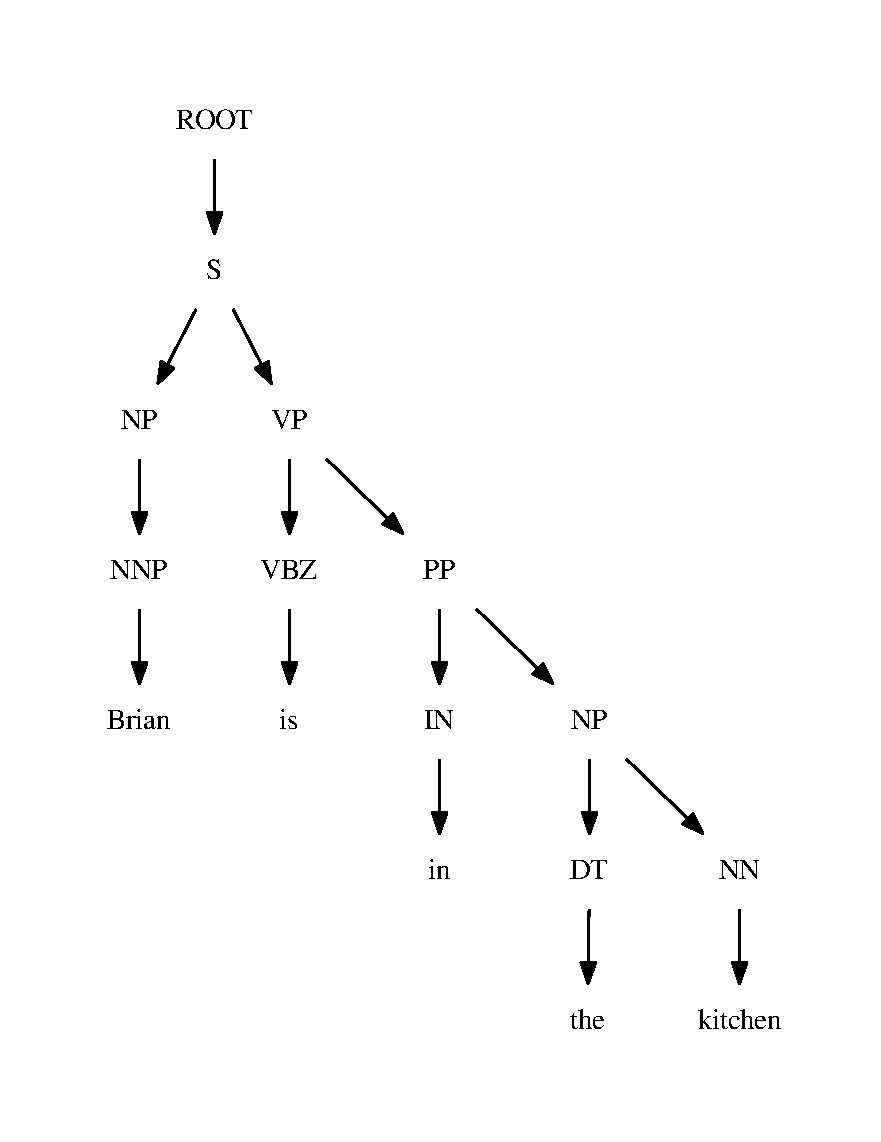
\includegraphics[scale=0.6]{../examples_NLP_grammatical/parsetree.pdf}
  \caption{Parse tree of \emph{Brian is in the kitchen.}}
  \label{ptree}
\end{figure}

\begin{figure}
  \centering
    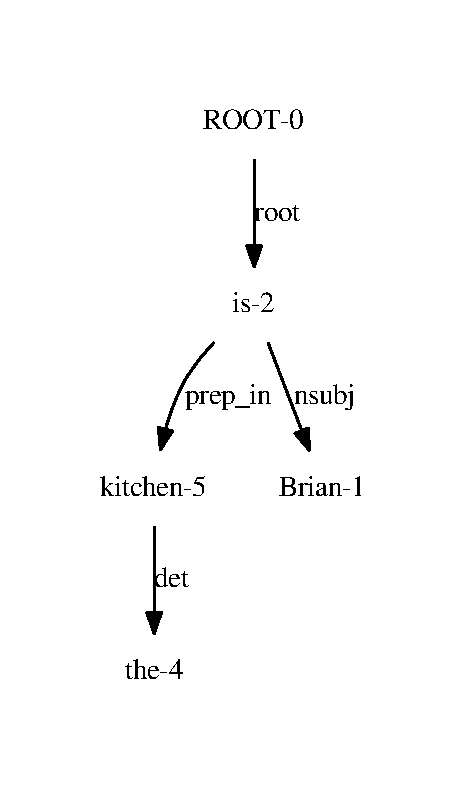
\includegraphics[scale=0.6]{../examples_NLP_grammatical/deptree.pdf}
  \caption{Dependency tree of \emph{Brian is in the kitchen.}}
  \label{dtree}
\end{figure}

We did not find a lot of detailed articles exposing procedures to get triples from the grammatical structure. For instance \cite{parsetree} tries to perform the extraction using the parse structure tree. However we believe the dependency tree could be more appropriate since it is more focused on the relations between the words than their roles in the sentence. Part \ref{gramap} presents an algorithm we have designed using the dependency tree representation.

We have also observed a growing use of machine learning techniques in NLP that try to automatically learn triples extraction rules instead of building intermediate grammatical representations. We will use such machine learning algorithms in parts \ref{mlreformulation} and \ref{mlwindow}.

The algorithms we focused on can handle factoid \textit{wh}-questions (i.e. closed-ended questions such as \textit{What is the capital of France}) and nominal sentences (e.g. \textit{capital of France}). 

Finally, some existing tools are very close to our goal.\footnote{\url{http://quepy.machinalis.com/}}\textsuperscript{,}\footnote{\url{http://www.ifi.uzh.ch/ddis/research/talking.html}}\textsuperscript{,}\footnote{\url{https://www.apple.com/fr/ios/siri/}}\textsuperscript{,}\footnote{\url{http://www.wolframalpha.com/}} They allow us to have a clear idea of the state of the art, and what performances in question answering we can expect.
